% \subsection{GPU Power Model is App Dependent}
% \label{subsec:gpu}

\paragraph{Parameters of the CPU and GPU power models}
Moto Z3~\cite{motoz3} is a representative modern smartphone
that uses the big.LITTLE CPU architecture~\cite{biglittlearch} to
provide energy efficiency in supporting diverse workloads.
Particularly, in Moto Z3, the LITTLE cores can operate in 22 different frequencies 
and big cores can operate in 31 different frequencies.
%  The cores are switched to higher frequencies when higher performance is required.
At runtime, the OS scheduler along with the CPU governor performs power state transition and core frequency scaling to optimize the CPU energy draw as the workload varies.
Thus the parameters of the CPU power model include
the base power consumed $p_{base}$ when the cores are idle and
the non-base core $i$ power running at frequency $f_k$, $p^c_i(f_k)$, as listed in Table~\ref{tab:parameters}.
The total CPU power can be modeled~\cite{multicoremodel:2015} as:
{
\begin{equation}
    P_{CPU} = p^c_{base} + \sum_{i} p^c_i(f_k)
\end{equation}

}

%\paragraph{Parameters of the GPU power model}
In Moto Z3, the GPU can run at 7 different frequencies and has three power states,
Active, Slumber (offline), and Aware.
% When the GPU is woken out of the Slumber state, it enters the Aware state for a brief duration.
% The Active state has two sub states, Active-busy when the GPU is computing and Active-idle
% when the GPU is idle. After staying in Active-idle for a threshold interval, the GPU enters the Slumber state.
Since the GPU never enters the Slumber or Aware state when an app is running, 
the parameters of the GPU model include only the GPU power draw in Active-busy and Active-idle states in each frequency, $p^g_{busy}(g_k), p^g_{idle}(g_k)$, as listed in Table~\ref{tab:parameters}.
We abbreviate Active-busy and Active-idle states simply
as GPU Busy and Idle states in the rest of the paper.

\if 0
Accordingly, we model the GPU power draw as follows:
\begin{equation}
    Power_{GPU} = \sum_{j}\sum_{i} u_{ij}*p_{ij}
    \end{equation}
where $p_{ij}$ is the power parameter for the $i^{th}$ GPU frequency for the $j^{th}$ power state (Active-busy, Active-idle, Slumber, Aware) and $u_{ij}$ is the corresponding utilization in that frequency and power state.
\fi

\paragraph{TPMD methodology}
We first derived CPU power models using microbenchmarks that perform arithmetic and memory operations for 7 seconds each 
with 100\% utilization.
We ran the microbenchmark while fixing the big core cluster at each of the 31 frequencies for both Pixel 2 and Moto Z3 and at each of the 17 frequencies for Pixel 4, 
on 1 core and 2 cores.
% When using 1 core, 2 cores and 4 cores, the remaining cores are offline.
We measure the base CPU power as the phone power draw when all cores are idle.
We manually align the power monitor readings for each of the 7-second interval 
and derive the non-base per-core power for each frequency by 
subtracting the base power from the measured total phone power.
{For the phones, we found that the per-core power $p_i(f_k)$ remains the same for different cores.}

% Similar to CPU, the GPU of modern smartphones have also vastly developed.
% Initially, we tried to use a GPU benchmark, 3DMark~\cite{3DMark}, to drive the GPU usage into Busy and Idle states under each frequency.
\begin{sloppy}
For the GPU, we found that GPU benchmarks, \eg 3DMark~\cite{3DMark}, typically render quite different consecutive frames which
result in rapidly fluctuating GPU utilizations and power monitor readings,
making the alignment difficult. 
\end{sloppy}
%
% This makes aligning the power monitor readings with the GPU Busy periods difficult
% which is needed to extract the GPU Busy state power at each frequency.
%
In contrast, we observe that real apps tend to render very similar consecutive frames in a short period of time which result relatively stable GPU utilization and stable total power draw, 
making it much easier to extract the power monitor reading corresponding to a given GPU utilization
(see Figure~\ref{fig:power_trace_candycrushturorial} later). 
%  the rendering task often finishes in less than the 16.7ms per-frame interval and hence the GPU will go through busy and idle states in every 16.7ms interval, making it much easier to manually identity both states. 
% \questionaj{Why do we have to identify manually? Triggers are not available in atrace?
% Due to both drift and scaling their is vast alignment problem in aligning each 16.7 ms interval.
% Alignment problem prevent us from directly using triggers from the event trace.}
Thus, we directly used selected apps that use only the CPU and GPU to derive the GPU power models. 
In particular, we 
derive the CPU model by first using the 
% integer-arithmetic 
CPU arithmetic microbenchmark\footnote{We found using the CPU model derived using memory-intensive microbenchmark resulted in negative GPU coefficients.} 
and then 
using the difference between the measured phone power and model-estimated CPU power when running an app  to determine the ground-truth for the GPU power draw and GPU power model derivation.


% 5. Explain results and observation

\begin{figure*}[tp]
    \centering
     \begin{subfigure}[b]{0.32\textwidth}
         \centering
         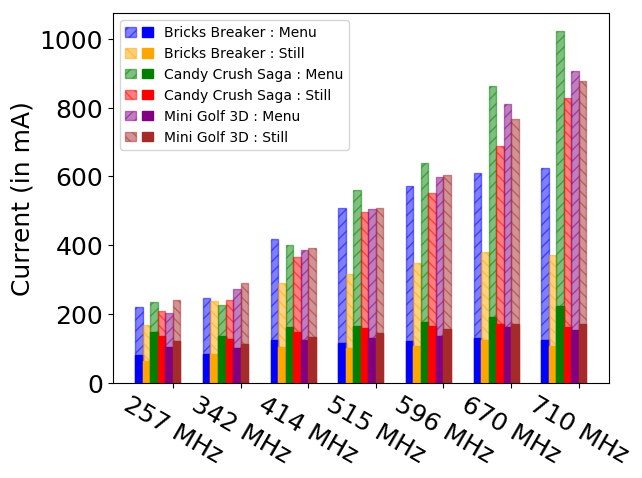
\includegraphics[width=\textwidth]{figures/002_Pixel2_gpu_model.png}
         \caption{Pixel 2}
         \label{fig:number_parameters_vs_duration_100s_0}
     \end{subfigure}
    \begin{subfigure}[b]{0.32\textwidth}
         \centering
         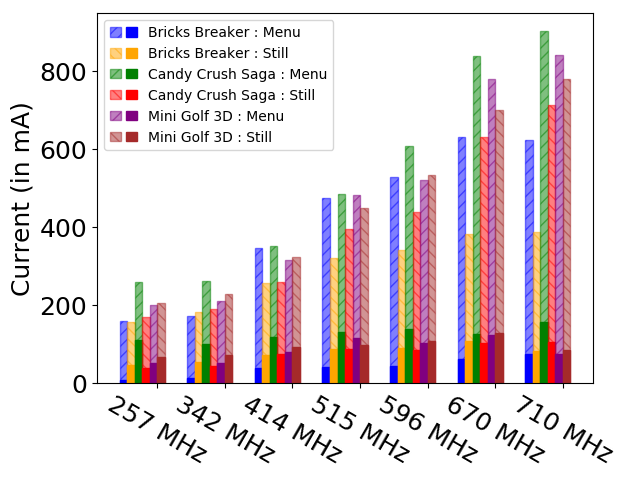
\includegraphics[width=\textwidth]{figures/003_MotoZ3_gpu_model.png}
         \caption{Moto Z3}
         \label{fig:number_parameters_vs_duration_100s_100}
     \end{subfigure}
    \begin{subfigure}[b]{0.32\textwidth}
         \centering
         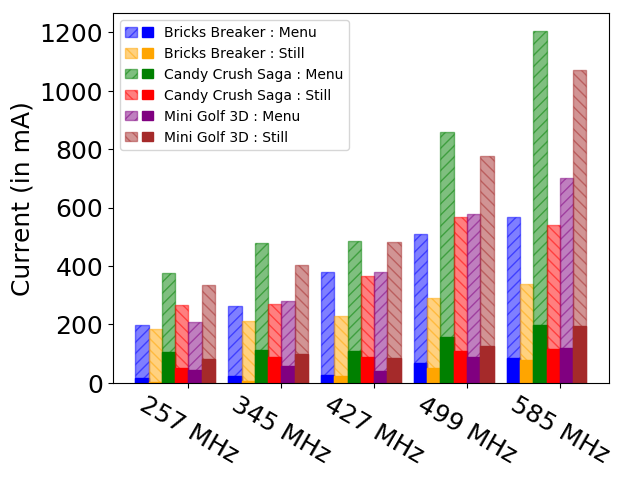
\includegraphics[width=\textwidth]{figures/004_Pixel4_gpu_model.png}
         \caption{Pixel 4}
         \label{fig:number_parameters_vs_duration_100s_200}
     \end{subfigure}
     \hfill
    \caption{GPU power model (Busy power in hatched and Idle power in solid) with the CPU fixed for the 3 phones.}
    \label{fig:gpu_model}
    \vspace{-0.1in}
\end{figure*}

\begin{table*}[]
    \caption{Energy estimation error (\%) for app scenarios 
    using the GPU model derived for each scenario with CPU and GPU fixed frequencies for the 3 phones. (B: Bricks Breaker, C: Candy Crush Saga and M: Mini Golf 3D)}
    \centering
     \begin{subfigure}[b]{0.32\textwidth}
        \centering
    	{ \scriptsize
    	\begin{tabular}{ | l | c | c | c | c | c | c | }
    		\hline
    		     & \multicolumn{6}{ c|}{Error for each App Scenarios (in \%)}\\
    		\cline{2-7}
                    Model & \rot{B. Menu} & \rot{B. Still} & \rot{C. Menu} & \rot{C. Still} & \rot{M. Menu} & \rot{M. Still}  \\
    		\hline
                B. Menu              & 8.9 & 13 & 20 & 16 & 11 & 14 \\
                B. Still             & 15 & 11 & 31 & 25 & 17 & 26 \\
                C. Menu              & 16 & 24 & 11 & 11 & 13 & 11 \\
                C. Still             & 16 & 19 & 14 & 12 & 12 & 14 \\
                M. Menu              & 9.9 & 14 & 14 & 11 & 8.1 & 11 \\
                M. Still             & 12 & 21 & 9.7 & 10 & 11 & 8.6 \\
    		\hline
    	\end{tabular}
    	}
	\caption{Pixel 2}
    \end{subfigure}
     \begin{subfigure}[b]{0.32\textwidth}
        \centering
    	{ \scriptsize
    	\begin{tabular}{ | l | c | c | c | c | c | c | }
    		\hline
    		     & \multicolumn{6}{ c|}{Error for each App Scenarios (in \%)}\\
    		\cline{2-7}
                    Model & \rot{B. Menu} & \rot{B. Still} & \rot{C. Menu} & \rot{C. Still} & \rot{M. Menu} & \rot{M. Still}  \\
    		\hline
                B. Menu              & 16 & 18 & 44 & 18 & 22 & 25 \\
                B. Still             & 18 & 15 & 36 & 15 & 17 & 17 \\
                C. Menu              & 30 & 24 & 16 & 23 & 18 & 16 \\
                C. Still             & 12 & 12 & 31 & 11 & 15 & 17 \\
                M. Menu              & 18 & 16 & 23 & 15 & 14 & 15 \\
                M. Still             & 20 & 15 & 20 & 14 & 12 & 13 \\
    		\hline
    	\end{tabular}
    	}
	\caption{Pixel 2}
    \end{subfigure}
         \begin{subfigure}[b]{0.32\textwidth}
        \centering
    	{ \scriptsize
    	\begin{tabular}{ | l | c | c | c | c | c | c | }
    		\hline
    		     & \multicolumn{6}{ c|}{Error for each App Scenarios (in \%)}\\
    		\cline{2-7}
                    Model & \rot{B. Menu} & \rot{B. Still} & \rot{C. Menu} & \rot{C. Still} & \rot{M. Menu} & \rot{M. Still}  \\
    		\hline
                B. Menu              & 15 & 15 & 44 & 19 & 15 & 34 \\
                B. Still             & 15 & 15 & 50 & 23 & 17 & 40 \\
                C. Menu              & 30 & 33 & 12 & 20 & 25 & 13 \\
                C. Still             & 18 & 20 & 25 & 15 & 16 & 19 \\
                M. Menu              & 15 & 16 & 34 & 17 & 14 & 26 \\
                M. Still             & 25 & 28 & 13 & 15 & 21 & 12 \\
    		\hline
    	\end{tabular}
    	}
	\caption{Pixel 2}
    \end{subfigure}
    \label{fig:gpu_model_error}
    \vspace{-0.1in}
\end{table*}
% Comparison Table for GPU model with other scenarios Here

We repeated the GPU model derivation for three
popular games apps, Bricks Breaker, Candy Crush Saga and Mini Golf 3D,
each running two scenarios, as listed in Table~\ref{tab:app_scenario_description}.
To minimize the variance of CPU power draw, we fixed the CPU frequency at 1.42 GHz for both Pixel 2,Moto Z3 and 1.61 GHz for Pixel 4,
and ran each of the app scenario under each GPU frequency for a duration of 30 seconds.

\paragraph{Derived model}
Our CPU modeling results (details omitted) show that
the CPU power draw for the arithmetic-intensive and memory-intensive
operations of the microbenchmark differ significantly,
by 38.7\% at the 300 MHz and 56.8\% at 2.45 GHz for Moto Z3.
This suggests that the arithmetic-memory operation mix can send the CPU cores
to different power state variations draining different power.
Figure~\ref{fig:gpu_model}(a)-(c) shows the derived GPU power models for varying GPU frequencies for the 3 phones. The full bars represent the busy current whereas the solid bars are the idle current.
% and Table~\ref{tab:gpumodel_nexus6} for Nexus 6.
%% 5a. Explain per scenario dependent modeling
From our findings we make two observations.
(1) The GPU power parameters for the same frequency differ with {\it different apps}; on Moto Z3 at 710 MHz, the GPU Busy power draw for Bricks Breaker Still is 57.2\% lower than for Candy Crush Saga Menu.
(2) The GPU power parameters for the same frequency even differ for {\it different scenarios} 
of the same app; for Bricks Breaker, the GPU Busy power draw
for the Still scenario is 32.3\% and 35.5\% lower than for the Menu scenario  at 515 MHz and 596 MHz respectively for Moto Z3.
Other phones also show simlar findings.

%% 5b. Explain the reasons for the observation
The above dependence of the GPU power draw on app usage can be attributed  to two main reasons.
First, the GPU has a large number of mini-cores, but the utilization metric available to the OS only captures the temporal utilization and not the spatial utilization, \ie the percentage of mini-cores those were active.
Different spatial utilization may drive the GPU into different power state variations that have the same temporal utilization but different power draw.


Second, using a single CPU model in estimating the CPU power draw which is to be subtracted from the total phone power may result in errors in the GPU power draw  estimation,
 as rendering different frames for different app scenarios (of the same or different apps) may result in different CPU usage, \eg due to different mix of arithmetic and memory operations and hence CPU power draw.
Such error propagation happens in TPMD which models one component at a time
and often relies on the models of a  prior component to estimate the "ground truth" in modeling  the next component. 

\paragraph{Cross validation}
To confirm that the GPU models derived per app scenario captures models dependence on the app usage also, we perform  a cross validation by applying
the GPU model derived from each of the six app scenarios shown in Figure~\ref{fig:gpu_model}(a)-(c)
and estimate the total energy of all app scenarios (including self). As shown in 
Figure~\ref{fig:gpu_model_error}(a)-(c) for the case where GPU frequency at 257 MHz  and CPU frequency 
fixed at 1.42 GHz for Pixel 2 and Moto Z3 and 1.61 GHz fixed for Pixel 4,
we observe that the error is the lowest when the GPU model specific to an app scenario is applied
to itself (same app scenario) i.e. the diagonal in the figure has the lowest error.
% \comment{
% We observe that the lowest error for a scenario is
% due to GPU model derived from same scenario (fitting error), whereas for
% all other scenario GPU models the error can be as much as 2$times$ higher.
% For the higher GPU frequencies, like 710 MHz the difference in the can increase up to about 10 times.
% }


\if 0
we calculated the error
in estimating the total GPU energy drain in the second scenario of each app 
if using the GPU model derived using the first scenario of each app.
The rows labelled "GPU energy error" in Table~\ref{tab:gpumodel_motoz3} shows that the error ranges between ??\%--??\%, ??\%--??\%, and ??\%--??\% for the second scenarios of the three apps.
\fi





